\documentclass[sigconf,anonymous,review]{acmart}

\usepackage{booktabs}
\usepackage{amsmath}
\usepackage{xspace}
\usepackage{pgfplots}
\pgfplotsset{compat=1.17}
\usetikzlibrary{decorations.pathreplacing}

\newcommand{\ic}{\mathrm{IC}\xspace}
\newcommand{\forgetic}{\ensuremath{\ic_{\mathcal{F}}}\xspace}
\newcommand{\Lzero}{\textsf{L0}\xspace}
\newcommand{\Lone}{\textsf{L1}\xspace}
\newcommand{\Ltwo}{\textsf{L2}\xspace}
\newcommand{\Lthree}{\textsf{L3}\xspace}
\newcommand{\gapclosed}{\ensuremath{\kappa}\xspace}

\settopmatter{printacmref=false}
\acmConference[ICAIF '26]{The 7th ACM International Conference on AI in Finance}{2026}{under review}
\setcopyright{none}

\begin{document}

\title[Can You Delete a Year of Market Data?]{Can You Delete a Year of
Market Data?\\ Machine Unlearning Against Exact Retraining Oracles}

\begin{abstract}
When a data license expires, its data must stop influencing
production models. Machine unlearning is the tool for this
obligation, but its ground truth, retraining from scratch without
the deleted data, is unaffordable at the scale the field studies,
so approximate methods are scored against proxies. Financial
forecasters retrain in minutes. We therefore evaluate deletion
against 3{,}200 exact retraining oracles on an S\&P~500 volatility
panel, spanning five architectures, five deletable years, three
deletion levels, and four test years. Three findings follow.
Deleting the COVID crisis year is not a cost. Every deployable
architecture forecasts the next bear market better without it, the
effect follows the deleted year's position in the training window,
and only the two architectures below a standard volatility
benchmark show no consistent response. The correct target of
unlearning is the counterfactual, not noise. The counterfactual
still predicts the deleted year at an information coefficient of
0.51, and forcing predictions toward noise surrenders the model. Of
twelve deployable architecture-method pairs, exactly one brackets
the oracle, at $74$--$118\%$ of its forgetting with skill intact,
and no ranking transfers across architectures or windows, so the
only trustworthy acceptance test is one's own oracle, which costs
minutes. Deletion is auditable only where the model memorized the
era. Seventeen per cent of legitimate deletions leave a trace too
faint to verify, window-level auditing stays near chance, and
treating overlapping windows as independent overstates audit
confidence. Protocol, code, and the full oracle--method--audit
matrix are released.
\end{abstract}

\maketitle

\section{Introduction}\label{sec:intro}

Quantitative finance runs on licensed data: vendor feeds, index
histories, alternative datasets. Licenses end. When one does, the
data must stop being used, including \emph{inside trained models}.
This is the problem machine unlearning addresses, and it arrives
here with a contractual rather than privacy motivation. The field's central obstacle is that
the ground truth of forgetting, retraining from scratch without the
deleted data, is unaffordable at LLM scale. Approximate methods are
therefore scored against
proxies~\cite{nguyen2025survey}, and the field's
verification tools are contested~\cite{zhang2024mia_cannot}.

Financial forecasters invert the economics: they retrain in minutes.
That affordability buys the study the field cannot run at scale. We
answer every question about unlearning against \emph{exact retraining
oracles}, 3{,}200 of them, on an S\&P~500 volatility-forecasting
panel, with every comparison paired by trading day.

One result reorganizes the rest. Deleting a clean, legitimate year of
market data is not a cost. In the next bear market it is a gain, and
the gain is largest for the models that memorized the year most. That
cuts against the long-tail account of memorization, in which
memorizing rare data is what buys generalization and removing it
should cost accuracy~\cite{feldman2020memorization}. Nothing is
wrong with the year we delete. What changes is the setting: a license
expires, the model is judged on a later regime, and under that shift
the value of a memorized era can invert. The unlearning literature
could not have found this. Approximate unlearning shows utility
falling, never rising. Seeing it rise takes the exact counterfactual,
which at this scale we can afford. Three research questions organize
the paper.

\textbf{RQ1: What does deleting a licensed era mean, and what does
exact deletion do?} \emph{Exact deletion is nearly inert in calm
markets, and under stress its sign is a property of the architecture,
not of the data.} First the question has to be made well-posed.
``Delete year $E$'' is not, because overlapping windows, rolling
features, and pipeline constants touch $E$ beyond its calendar
bounds. We formalize a membership lattice of four increasingly
strict readings and adopt the window-level reading as the
paper-wide default. Measured against oracles, deletion moves a calm
test year by almost nothing. In the next bear market the same
deletion moves an order of magnitude more, and every deployable
architecture gains from removing the crisis year. The two
architectures below a standard volatility benchmark do not gain,
and they are the two no one should deploy. Deletion exposure is
therefore something to screen for, not a fixed cost to budget.
Within a single training window, the effect follows the deleted
era's position. The earliest years are inert, the years just before
the test period cost skill, and deleting the crisis year helps.

\textbf{RQ2: Can approximate unlearning substitute for retraining,
and what is the right target?} \emph{The right target is the
counterfactual, and the counterfactual still predicts the deleted
era.} The only prior forecasting-specific
method~\cite{wang2026tsunlearn} drives forgotten predictions toward
noise. Yet the counterfactual, retrained without the crisis year,
still predicts that year almost as well as the reference, because
nearly all of that skill is generalization rather than memory.
Approaching the noise target therefore surrenders live skill.
Compliance means matching the counterfactual. On substitution the
answer is no. In a single fold several deployable
architecture-method pairs look adequate. Across all four folds,
exactly one brackets the oracle, one more stays within half the
gap, and the rest under-forget or overshoot.

\textbf{RQ3: Can deletion be audited?} \emph{Only when the model
memorized the era. Auditability is a property of what was learned, not
of what was deleted.} An auditor calibrated against a population of
retrainings separates crisis-era deletions easily, but across the
full grid the separation falls to chance, and seventeen per cent of
legitimate deletions leave a trace too faint to verify. A null
audit is therefore not evidence of compliance. Window-level
auditing stays near chance everywhere, and treating overlapping
windows as i.i.d.\ overstates audit confidence. Audit granularity
belongs in the data contract.

\textbf{Contributions.} (i)~The sign result: exact deletion of a
crisis era improves every deployable architecture in all four
market regimes, and the sign is carried by the architecture, not by
the data. (ii)~The instrument: 3{,}200 exact retraining oracles and
the full oracle--method--audit matrix, released for reuse. (iii)~A
membership lattice that makes ``delete year $E$'' well-posed under
overlapping windows, with measurements of what each reading costs
in data and in measured memory. (iv)~The target result: the
counterfactual still predicts the deleted era, so compliance and
privacy forgetting are different objectives, and pursuing the
second surrenders the model. (v)~The audit result: audit strength
tracks what the model memorized, not what was deleted, so
legitimate deletions can be unverifiable at any granularity.

\section{Related Work}\label{sec:related}

\textbf{Machine unlearning.} The problem dates to Cao and
Yang~\cite{cao2015towards}, and the GDPR right to
erasure~\cite{gdpr2016} gave it urgency. The families are exact
unlearning by training-time design~\cite{bourtoule2021sisa} and
approximate post-hoc editing by gradient ascent, relabeling or
distillation~\cite{kurmanji2023scrub}, mapped by
surveys~\cite{nguyen2025survey}.
Evaluation increasingly treats the retrained model as ground
truth~\cite{shi2024muse}, but at scale the oracle
stays unaffordable and proxies dominate. We invert that constraint
and instantiate the oracle for every question asked.

\textbf{Unlearning for time series.}
TS-Unlearn~\cite{wang2026tsunlearn} is to our knowledge the only
forecasting-specific method, a teacher--student scheme whose forget
objective drives predictions toward Gaussian noise. Its authors
read forget error exceeding the retrained reference as
thoroughness, a privacy framing, and note qualitatively that
autocorrelation lets retained data inform forgotten samples. We
measure how far the noise target sits from the compliance one, and
our membership lattice turns their observation into a definition.

\textbf{Auditing and membership inference.} Membership inference
attacks test whether a datum was in a model's training set,
calibrated against ``shadow'' models trained with and without it.
They are the standard verification
primitive~\cite{carlini2022lira}, and their limits are
contested~\cite{zhang2024mia_cannot}. The time-series
adaptations partition members by
individual~\cite{johansson2026privacy}, which sidesteps the
overlapping-window ambiguity. Temporal forget units make that
ambiguity unavoidable, and our audit design confronts it directly.

\textbf{Is memorized data worth keeping?} Two literatures answer
this, each under an assumption our setting does not grant.
Long-tail theory shows that memorizing rare examples is necessary
for generalization under i.i.d.\
evaluation~\cite{feldman2020memorization}. Data valuation finds
subsets worth dropping without retraining, but the subsets it
surfaces are corrupted or
mislabelled~\cite{ghorbani2019datashapley}. We use the era-level
analogue of the per-example memorization
score~\cite{feldman2020what} throughout.

% [PAGE-BUDGET L3] restore by removing the leading %% on this block
%\textbf{Evaluation at financial signal-to-noise.} Financial forecast
%evaluation has its own discipline: signal-bearing tasks, paired daily
%tests with HAC standard errors~\cite{newey1987hac}, and
%minimum-detectable-effect accounting. Without it, degradation and
%forgetting claims at this signal-to-noise are unfalsifiable. We adopt
%it wholesale, and it is not optional: i.i.d.\ treatment of
%overlapping windows materially overstates audit confidence.

\section{Methodology}\label{sec:method}

\subsection{The unlearning problem}

Machine unlearning arises when part of a model's training data must
be deleted after training. Let $D$ be the training data and $A$ the
training procedure, including the architecture, the hyperparameters,
and the random seed. The \emph{forget set} $F \subset D$ holds the
observations to be deleted, and the \emph{retain set} $D \setminus F$
holds the rest. The model trained on everything, $A(D)$, is the
\emph{reference}. The model retrained from scratch on the retain
set, $A(D \setminus F)$, is the \emph{oracle}, or
\emph{counterfactual}, the ground truth of deletion. Because
retraining is often unaffordable, \emph{approximate unlearning}
instead edits the reference in place with an \emph{unlearning
operator} $U$, aiming for a model that a prescribed audit cannot
distinguish from the oracle.

\begin{table}[t]
\centering
\caption{Deletion levels for a requested period $T$. Each level
includes all restrictions of the preceding level. \Lone{} is the
paper-wide default.}
\label{tab:deletion_levels}
\footnotesize
\begin{tabular}{@{}p{0.13\columnwidth}p{0.78\columnwidth}@{}}
\toprule
Level & Prohibited use of $T$ and representative examples \\
\midrule
\Lzero{} &
\textbf{Target deletion.}
Use in forecast targets, such as prediction labels. \\
\Lone{} &
\textbf{Window deletion.}
Direct appearance in inputs or targets, such as context windows,
and use in the normalization statistics that scale them. \\
\Ltwo{} &
\textbf{Derived-data deletion.}
Dependence through feature construction, such as rolling statistics
and imputation. \\
\Lthree{} &
\textbf{Full-pipeline deletion.}
Influence on model-development decisions, such as hyperparameter
tuning and model selection. \\
\bottomrule
\end{tabular}
\end{table}

\subsection{A membership lattice for temporal deletion}

In time series, a deletion request does not name a forget set. It
names a period $T$, a set of dates whose use is no longer permitted.
A single date inside $T$ can touch a rolling forecaster in four
distinct ways, and each way is one level of
Table~\ref{tab:deletion_levels}. Consider one trading day in March
2020. It is the prediction \emph{target} of the windows that
forecast it (\Lzero). It sits inside the 64-day \emph{input context}
of windows whose targets fall up to three months later (\Lone). It
enters \emph{derived quantities} computed from it, such as rolling
features with long tails (\Ltwo). And it may have influenced
\emph{model-development decisions} such as hyperparameter tuning
(\Lthree). Each level forbids everything the preceding level does
plus one further form of dependence, so the four readings are
nested. We call this ordering the membership lattice. The first
three levels change only which training examples are retained,
giving nested forget sets $F_\ell(T)$, whose exact construction is
specified in the released protocol.

Strictness has a measurable price in two currencies. The first is
data. Because windows overlap, \Lone{} removes windows whose target
dates lie outside $T$, and on this panel it surrenders about $25\%$
more windows than \Lzero. The second is the measurement itself. The
level changes the forget set, and with it the measured memorization
gap (Section~\ref{sec:levels}). A temporal deletion request is therefore incomplete unless its
level is named. We adopt \Lone{} as the paper-wide default and use
\Lzero{} and \Ltwo{} as robustness checks. \Lthree{} may alter the
training procedure itself rather than only the retained examples.
It coincides with \Ltwo{} here by construction, because tuning and
model selection predate every deletable era.

At every level, the target of unlearning is the oracle retrained
without that level's forget set,
\begin{equation}
U\!\left(A(D),F_\ell(T)\right)
\;\approx_d\;
A\!\left(D\setminus F_\ell(T)\right),
\qquad
\ell\in\{0,1,2\},
\label{eq:unlearning}
\end{equation}
where $\approx_d$ is approximate equality in distribution under a
prescribed audit, and the method and the oracle use the same level.

% [PAGE-BUDGET L1] restore by removing the leading %% on this block
%\begin{figure}[t]
%\centering
%\begin{tikzpicture}[x=0.68cm, y=0.5cm, font=\footnotesize]
%  \fill[gray!20] (3.2,-3.95) rectangle (5.6,0.55);
%  \draw[gray!60] (3.2,-3.95) rectangle (5.6,0.55);
%  \node at (4.4,-0.05) {deleted era $T$};
%  \draw[decorate, decoration={brace, amplitude=3pt}]
%    (5.65,0.55) -- (6.95,0.55) node[midway, above=3pt] {context halo};
%  \draw[->] (0,-3.95) -- (8.3,-3.95);
%  \node[below] at (4.15,-3.95) {trading days};
%  \node[right] at (8.0,-0.15) {dropped at:};
%  \draw[fill=gray!8] (0.2,-1.10) rectangle (1.60,-0.65);
%  \fill[black] (1.60,-1.10) rectangle (1.78,-0.65);
%  \node[right] at (8.0,-0.875) {---};
%  \draw[fill=gray!8] (1.75,-1.75) rectangle (3.15,-1.30);
%  \fill[black] (3.15,-1.75) rectangle (3.33,-1.30);
%  \node[right] at (8.0,-1.525) {\Lzero{}, \Lone};
%  \draw[fill=gray!8] (3.50,-2.40) rectangle (4.90,-1.95);
%  \fill[black] (4.90,-2.40) rectangle (5.08,-1.95);
%  \node[right] at (8.0,-2.175) {\Lzero{}, \Lone};
%  \draw[fill=gray!8, very thick] (4.70,-3.05) rectangle (6.10,-2.60);
%  \fill[black] (6.10,-3.05) rectangle (6.28,-2.60);
%  \node[right] at (8.0,-2.825) {\Lone{} only};
%  \draw[fill=gray!8] (6.30,-3.70) rectangle (7.70,-3.25);
%  \fill[black] (7.70,-3.70) rectangle (7.88,-3.25);
%  \node[right] at (8.0,-3.525) {---};
%\end{tikzpicture}
%\caption{One deletion request, four readings. Each row is a training
%window: bar $=$ 64-day context, dark tick $=$ 5-day forecast target.
%\Lzero{} drops windows whose \emph{target} touches $T$ (rows 2--3).
%\Lone{} also drops windows whose \emph{context} touches $T$ (row 4,
%bold). Row 5 lies beyond the halo and survives both.}
%\label{fig:lattice}
%\end{figure}

\subsection{Counterfactuals and governance metrics}

For each deletion request and level, the oracle retrains the model from
scratch on the retain set under the reference model's training
protocol. An approximate method is judged by how closely it reproduces
this counterfactual, not by how much it degrades predictions on the
deleted period.

Let $\text{ref} = A(D)$ denote the reference model,
$\text{ora} = A(D \setminus F_\ell(T))$ the retrained counterfactual,
and $m = U(\text{ref}, F_\ell(T))$ the model produced by an approximate
operator. The forget-set loss $\mathcal{L}_F(\cdot)$ measures how
well a model still fits the deleted data, so a higher loss indicates
more forgetting. The test score $s_{\text{test}}(\cdot)$
measures forecast quality on the test set, oriented so that higher is
better.

\textbf{Memorization gap $G_F$.} The memorization gap is the reference
model's excess fit over the counterfactual on the forget set,
\begin{equation}
G_F = \mathcal{L}_F(\text{ora}) - \mathcal{L}_F(\text{ref}).
\label{eq:gap}
\end{equation}
A gap near zero means the forget set was barely memorized; a large gap
means it was memorized strongly. $G_F$ is the era-level analogue of the per-example memorization
score of Feldman and Zhang~\cite{feldman2020what}. It carries the
units of the target a model was fit to, and is rescaled as
$G_F/\mathrm{Var}(y_T)$ when a model with a different target is
compared.

\textbf{Closure $\gapclosed$.} The closure is the fraction of the
memorization gap that a method $m$ removes,
\begin{equation}
\gapclosed(m) =
\frac{\mathcal{L}_F(m) - \mathcal{L}_F(\text{ref})}{G_F}.
\label{eq:kappa}
\end{equation}
A closure of $0$ means the method forgets nothing and remains at the
reference, $1$ means it reaches the counterfactual, and above $1$
means it over-forgets.

\textbf{Deletion effect $\Delta s_{\text{test}}$.} The deletion effect
is the change in test score caused by exact deletion, measured one day
at a time so that offsetting daily differences are not hidden by the
average. The reference and the counterfactual score the same
cross-section on each evaluation day $t$, so the daily change is
$\Delta s_t = s_t(\text{ora}) - s_t(\text{ref})$, and
\begin{equation}
\Delta s_{\text{test}} =
\frac{1}{N_{\text{test}}}\sum_{t=1}^{N_{\text{test}}} \Delta s_t .
\label{eq:delta}
\end{equation}
A positive $\Delta s_{\text{test}}$ means deletion improves the
test score, and a negative value means the deleted period carried
useful signal. Where no confusion arises we write $\Delta$ for
$\Delta s_{\text{test}}$ and $G$ for $G_F$.

\subsection{Auditing deletion}

The goal of an audit is to determine whether information from the
deleted period remains detectable in the model. Throughout,
\emph{verified} means one thing only: detectors of stated power found
no gap above their minimum detectable effect. It never means proof
that no trace remains.

The audit forms two populations by retraining under different random
seeds: references that include $T$ in training, and counterfactuals
that omit it. This is the access model a model owner or an appointed
auditor can realistically arrange: fixed code, fixed data cuts, and
multiple retraining seeds. Given a per-model statistic $a(\cdot)$,
the audit separation is
\begin{equation}
d' = \frac{\bigl\lvert\, \overline{a(\text{ora})} -
\overline{a(\text{ref})} \,\bigr\rvert}{\mathrm{sd}_{\text{pool}}},
\label{eq:dprime}
\end{equation}
the standardized distance between the two population means, where
$\mathrm{sd}_{\text{pool}}$ is the pooled standard deviation across
seeds. A large $d'$ means the populations separate and deletion is
detectable; $d' \approx 0$ means they are indistinguishable and
deletion cannot be certified from $a$. We take $a = \mathcal{L}_F$
because it is evaluated on the deleted data, where the populations
separate sharply. We report $d'$ rather than an AUC because $d'$
does not saturate.

The granularity of $a$ matters. Aggregating over the whole deleted
period gives an era-level audit, and scoring individual overlapping
windows gives a window-level audit.

\section{Experimental Setup}\label{sec:exp}

\subsection{One run of the study}

We train a Transformer on the five years 2016--2020 and deploy it on
2022. Now the license on the 2020 data expires. We retrain the same
architecture, with the same hyperparameters and the same seed, on the
remaining four years. The original model is the reference of Section~\ref{sec:method},
and the retrained one is the oracle. This one pair answers every
question in the paper. Its fit gap on 2020 is the memorization gap
$G$, its forecast difference on 2022 is the deletion effect
$\Delta$, and whether an auditor can tell the pair apart is the
audit question.

The full study repeats this comparison 3{,}200 times. One
combination of architecture, training window, deleted year, and
deletion level is a \emph{cell}, with ten seeds per cell. Five
architectures, four windows, five deletable years, three levels,
and ten seeds give 3{,}000 oracle retrains, and a placebo control
adds 200.

\subsection{Forecasting task and data}

The task is 5-day-ahead realized volatility for S\&P~500 stocks, one
cross-section per trading day: each day the model ranks stocks by how
volatile the next five days will be. This is a risk task rather than
an alpha contest; the ranking feeds volatility targeting and position
sizing. For each asset $i$ and day $t$ the model reads a 64-day
history of eleven return-derived features and predicts
$y^{\mathrm{raw}}_{i,t} = \log
\operatorname{sd}\{r_{i,t+1},\ldots,r_{i,t+5}\}$, the log
volatility of its next five daily returns, $z$-scored within each
day's cross-section and clipped to $[-3,3]$. Training minimizes
mean squared error against this target.

Daily returns are dividend- and split-adjusted simple returns for a
fixed list of 501 current S\&P~500 constituents, so delisted firms
are excluded by construction. The panel covers 2015--2025, about
480 stocks per day, and hyperparameter tuning uses an earlier
extract reaching back to 2008. The panel and its construction
scripts are released.

\subsection{Rolling windows and deletions}

There is one training design, not four: a five-year window slid
forward one year at a time. Each position of the window validates
on the following year and tests on the year after that. We call
each window position a \emph{fold}, named by its test year: the
2022 fold trains on 2016--2020, validates on 2021, and tests on
2022, and the folds run through 2025. Rolling fixed-width windows
are standard deployment practice and give every era a scheduled
exit, which makes deleting a year still inside the active window
the live compliance case.

Sliding the window is also what separates the paper's two questions.
Within one window position, the deleted year varies while the test
year is held fixed. Across window positions, the same deleted year
(2020, the crisis) is removed under four different test years. The
first isolates what was deleted, and the second isolates the market
it is judged in.

Two controls complete the design. A \emph{random-deletion placebo}
removes the same number of windows as the 2020 deletion, drawn
uniformly, and separates the effect of losing data volume from the
effect of losing that particular year. We deliberately do not top up
the training set to equalize volume, because the compliance
counterfactual of an expiry is a smaller training set.

\subsection{Models and benchmark}

We tune seven forecasting backbones and report the five that span the
fit range: the vanilla Transformer~\cite{vaswani2017attention},
TSMixer~\cite{chen2023tsmixer}, SegRNN~\cite{lin2023segrnn},
iTransformer~\cite{liu2024itransformer}, and
PatchTST~\cite{nie2023patchtst}. Two further backbones fit worse
than the weakest of these and add no further contrast, so they
appear only in the released sweep.

As an econometric benchmark we refit the heterogeneous autoregressive
(HAR) model of realized volatility~\cite{corsi2009har} under the
identical protocol: log 5-day-forward realized volatility regressed
on its trailing 1-, 5-, and 22-day counterparts by ordinary least
squares. It has four parameters, is subject to the same deletions,
and sets the line the results are organized around: a neural
forecaster that cannot beat it has no business in production. We call
the three architectures that beat it in every fold the
\emph{deployable} models. The two that never do underfit this task,
and we call them the \emph{non-deployable} models.

\subsection{Metrics, tuning, and cost}

Forecast skill is the daily cross-sectional information coefficient
(IC): each day, the Spearman rank correlation between predictions and
targets across stocks, averaged over the test year's days,
written $s_{\text{test}}$. The same quantity computed on the deleted
year's windows is written \forgetic{}. The forget-set loss
$\mathcal{L}_F$ is the mean squared error on those windows. The
governance metrics $G$, $\Delta$, and $\gapclosed$ of
Eqs.~\ref{eq:gap}--\ref{eq:kappa} are built from these. Every
comparison is paired by trading day with Newey--West standard
errors~\cite{newey1987hac}, forget-set metrics are means over ten
seeds, and the audit separation $d'$ compares the two ten-seed
populations.

Hyperparameters were tuned once, on a split that predates every
deletable year (2010--2014, validated on 2015, disjoint seeds),
selecting on validation loss over a grid of width and dropout. A second search over learning rates and structural
settings changed nothing. iTransformer and
PatchTST remain below the HAR benchmark after that dedicated search,
so their weak fit is a property of the architecture on this task, not
of the tuning budget. A single oracle retrain costs 3--18 minutes on
one NVIDIA A100, and the full campaign took about 600 A100-hours.
Full configurations are in the released protocol.

\section{RQ1: What Does Exact Deletion Do?}\label{sec:rq1}

This section compares the reference model of Section~\ref{sec:exp},
trained on the full five-year window, with the oracle, retrained
after one training year is removed. The comparison produces two
quantities, measured on different parts of the data.

The memorization gap $G$ (Eq.~\ref{eq:gap}) is measured on the
removed year. It is the oracle's forecast error on that year minus
the reference's error on the same year. The reference trained on the
year and the oracle did not, so a large gap means that fitting the
year required training on it. $G$ therefore measures how much of the
year the model memorized.

The deletion effect $\Delta$ (Eq.~\ref{eq:delta}) is measured on the
test year. It is the oracle's forecast skill minus the reference's
skill. Neither model trained on the test year, so $\Delta$ measures
what the deletion does to subsequent forecasts. A positive $\Delta$
means the model forecasts better without the removed year. We report
$G$ first, then $\Delta$, and finally how both depend on which year
of the window is removed.

Tables~\ref{tab:years} and~\ref{tab:skill} provide the context for
these results. Table~\ref{tab:years} summarizes the market conditions
of each year. The COVID crisis year 2020 is by far the most volatile
year in the sample, with $38\%$ realized volatility, compared with
$24\%$ in the 2022 bear market and $7$--$18\%$ in the low- to
medium-volatility years.
Table~\ref{tab:skill} reports the test skill of the five
architectures. The deployable models, the Transformer, TSMixer, and
SegRNN, exceed the HAR benchmark in every fold. The non-deployable
models, iTransformer and PatchTST, never do. Both distinctions, the
crisis year against the low- to medium-volatility years and the
deployable models against the non-deployable ones, recur throughout
the results.

\begin{table}[t]
\caption{Realized volatility of the deletable years
(equal-weighted panel); each sits inside at least one training
window. 2020 is the COVID crisis, 2022 the bear market, and the
remaining years are low- to medium-volatility years. The test
years' volatilities appear with the fold results.}
\label{tab:years}
\centering
\setlength{\tabcolsep}{3.6pt}
\footnotesize
\begin{tabular}{lcccccccc}
\toprule
Year & 2016 & 2017 & 2018 & 2019 & \textbf{2020} & 2021 & 2022 & 2023\\
\midrule
Realized vol.\ (\%) & 14 & 7 & 16 & 13 & $\mathbf{38}$ & 14 & 24 & 14\\
\bottomrule
\end{tabular}
\end{table}

\begin{table}[t]
\caption{Reference skill (IC) per fold. Rows are sorted by skill,
and the refitted HAR benchmark, evaluated on the same test years,
separates the deployable models above it from the non-deployable
models below it. Folds are ordered by test-year volatility.}
\label{tab:skill}
\centering
\setlength{\tabcolsep}{5pt}
\footnotesize
\begin{tabular}{lcccc}
\toprule
& 2022 & 2025 & 2023 & 2024\\
Architecture & ($24\%$) & ($18\%$) & ($14\%$) & ($12\%$)\\
\midrule
Transformer & $0.570$ & $0.454$ & $0.470$ & $0.489$\\
TSMixer & $0.560$ & $0.463$ & $0.458$ & $0.488$\\
SegRNN & $0.517$ & $0.452$ & $0.441$ & $0.476$\\
\midrule
HAR (benchmark) & $0.508$ & $0.412$ & $0.384$ & $0.396$\\
\midrule
iTransformer & $0.125$ & $0.213$ & $0.174$ & $0.221$\\
PatchTST & $0.168$ & $0.181$ & $0.181$ & $0.169$\\
\bottomrule
\end{tabular}
\end{table}

\begin{figure}[t]
\centering
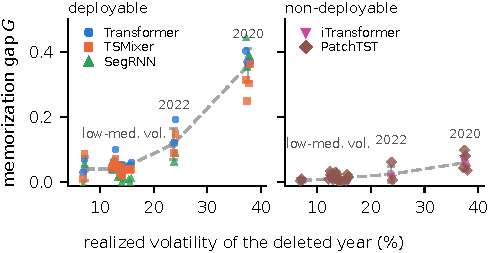
\includegraphics[width=0.92\columnwidth]{figs/fig_gap}
\caption{Memorization gap $G$ for all 100 cells (5 architectures
$\times$ 4 folds $\times$ 5 deleted years, \Lone; each point the
mean of 10 seeds), placed at the realized volatility of the deleted
year and jittered horizontally by fold. Left: the three deployable
architectures. Right: the two non-deployable ones, on the same
vertical scale. The grey dashed curve connects the means of the
four volatility clusters, bars $\pm 1$ sd.}
\label{fig:gap}
\end{figure}

\subsection{Memorization of training years}

Figure~\ref{fig:gap} shows the memorization gap for every combination
of architecture, fold, and deleted year. Each point is placed at the
realized volatility of the deleted year. The gap increases with
volatility for every architecture. Deleting 2020 produces the largest
gap in every fold, the low- to medium-volatility years produce gaps
near zero, and the 2022 bear year lies between the two. Models therefore memorize
volatile years far more strongly than calm ones.

The size of the gap depends on model capacity. For every deleted
year, the three deployable architectures (left panel) show
gaps several times larger than the two non-deployable ones (right
panel). The
HAR benchmark shows the same pattern at a much smaller magnitude. The
volatility of a year determines whether it is memorized, and model
capacity determines how strongly.

A plausible explanation is the absence of substitutes. A model
trained without 2019 can still fit 2019, because the remaining calm
years contain similar dynamics. A model trained without 2020 cannot
reconstruct the crisis from the remaining years, because none of them
resembles it. Two controls support this interpretation. A placebo
deletion that removes the same number of training windows at random
produces no gap, and the gap is unrelated to how well the reference
model fits each year. The gap therefore reflects the content of the
deleted year, not the amount of data removed and not the difficulty
of the year.

\begin{figure}[t]
\centering
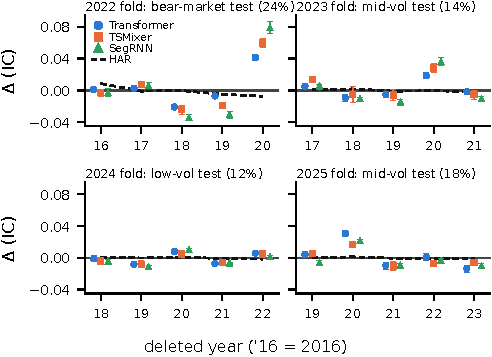
\includegraphics[width=0.92\columnwidth]{figs/fig_ladder}
\caption{Deletion effect $\Delta$ of removing each training year,
in every fold (\Lone, 10 seeds per point, bars $\pm 1$ standard
error; all panels share one scale; points offset slightly for
visibility). The dashed black line is the refitted HAR benchmark.
The two non-deployable architectures share no common shape and are
omitted.}
\label{fig:ladder}
\end{figure}

\subsection{Effect of deletion on forecast skill}

Figure~\ref{fig:ladder} reports the deletion effect for the three
deployable architectures. Each panel corresponds to one
fold, and each point gives the change in test-year skill caused by
deleting one training year. A positive value means that the model
forecasts better without that year. Deleting 2020 improves all three
architectures in all four folds. The improvement is largest in the
2022 fold, whose bear-market test year is most similar to the
deleted crisis, and it decreases as the test year becomes calmer. In
the 2024 fold, which has the lowest-volatility test year, no
architecture
changes by more than about $3\%$ of its skill, an amount close to
the placebo effect. The most strongly memorized year is therefore
also the only year whose deletion consistently improves forecasts.

If the 2020 observations were simply misleading about later markets,
every model should improve when they are removed. The HAR benchmark,
subjected to the identical deletion (dashed line in each panel),
instead loses a small amount of skill. The benchmark has too little
capacity to memorize the crisis and extracts useful information from
the 2020 data. The improvement therefore reflects a property of the
deployable models, not a defect of the data. Prior work shows
that memorizing atypical examples improves test accuracy when
training and test distributions
coincide~\cite{feldman2020memorization}. In our setting the test
regime differs from the memorized one, and memorization reduces
accuracy instead. The data cannot identify which property of the
deployable models drives the improvement, because test skill and
memorization increase together across the five architectures. The
effect is not specific to a single architecture. TSMixer was added
after the experimental design was fixed, its improvement under the
2020 deletion was predicted in advance, and the prediction was
confirmed.

The two non-deployable architectures show no comparable
regularity. Their deletion effects change sign across folds and
deletion levels, and PatchTST loses about $40\%$ of its skill in the
bear-market fold. The HAR benchmark therefore also functions as a
screening criterion. The deployable models respond to deletion
consistently, and the non-deployable models do not. The gains
are also not carried by a few turbulent days. The oracle
outperforms the reference on the majority of individual test days.

\subsection{Dependence on the position of the deleted year}

Comparing the five deletions within each panel of
Figure~\ref{fig:ladder} shows that the position of the deleted year
matters. Deleting the earliest years of a window has almost no
effect. Deleting the low- to medium-volatility years immediately
before the test period reduces skill. Deleting the crisis year improves skill at
every position in the window. As the window slides forward, this
pattern moves with it.

We do not have a complete explanation for this pattern. The most
natural hypothesis is that a deletion helps when it makes the
training distribution more similar to the test year. The data
contradict it. The 2020 deletion shifts the training distribution
furthest from the test year, yet it is the only deletion that helps.
The results support two more limited conclusions. Recent low- to
medium-volatility years contain information that the models still
use, and a crisis year can degrade a high-capacity model once its
regime has passed.
Both effects are present within a single training window, and which
one a given deletion produces cannot be predicted from the data
alone. The retraining oracle measures it directly.

\subsection{Dependence on the deletion level}\label{sec:levels}

\begin{table}[t]
\caption{Price and measurement at each deletion level. Each
stricter reading of ``delete 2020'' is measured against its own
oracles. Data cost is the share of training windows surrendered,
$G(2020)$ is the memorization gap of the Transformer averaged over
folds and seeds, and the last column is the delete-2020 effect
across the twelve deployable cells. \Lone{} is the paper-wide
default.}
\label{tab:levels}
\centering
\footnotesize
\begin{tabular}{llcc}
\toprule
Level & Data cost & $G(2020)$ & Delete-2020 effect \\
\midrule
\Lzero & $20\%$ of windows & $0.527$ & $12/12$, all significant \\
\Lone & $+25\%$ windows & $0.375$ & $12/12$, all significant \\
\Ltwo & a further $+2\%$ & $0.368$ & $12/12$, $11$ significant \\
\bottomrule
\end{tabular}
\end{table}

Every result so far reads the deletion request at \Lone. The grid
repeats each deletion at \Lzero{} and \Ltwo{} with the same ten
seeds, so the price of strictness is measured rather than assumed.
Table~\ref{tab:levels} summarizes what the level changes.

Measured memory moves most. The crisis-year gap falls at each
stricter reading, in all twenty architecture-fold cells. The forget
sets are nested, so this decline means the windows each stricter
level adds carry smaller gaps than the crisis core. Nearly all of
the decline occurs in the step from \Lzero{} to \Lone, the step
that adds the overlapping context windows and recomputes
normalization. The further step to \Ltwo{} barely moves the gap. The gaps of the
low- to medium-volatility years move by less and in directions that
depend on the year. Two contracts naming the same period at
different levels therefore measure different amounts of memory.

No conclusion of this section changes direction with the level.
Deleting 2020 helps every deployable architecture at every level,
in all twelve cells, and only at \Ltwo{} does one cell lose
statistical significance. The losses from deleting the years just
before the test period are confirmed at \Lzero{} in the bear-market
fold, so they are not an artifact of the wider \Lone{} forget set.
The non-deployable models are not even stable across readings.
iTransformer's delete-2020 effect is positive at \Lzero{} and
vanishes at \Lone. \Lthree{} coincides with \Ltwo{} by
construction. The deletion level is a genuine contract parameter.
It changes what a deletion costs and how much memory it measures,
but not the direction of any finding. RQ2 asks whether retraining,
at whatever level the contract names, can be avoided.

\section{RQ2: Can Retraining Be Avoided, and What Is the Target?}
\label{sec:rq2}

An approximate unlearning method edits the reference model in place
instead of retraining it. This section asks whether an edited model
can substitute for the oracle. The question has two parts, and the
order matters. A method can only be judged against a target, so we
first establish what forgetting should aim at. We then measure how
close four methods come to that target.

Closeness is measured by the closure $\gapclosed$
(Eq.~\ref{eq:kappa}), evaluated on the removed year. A closure of
$0$ means the edited model still fits the removed year as well as
the reference, so nothing was forgotten. A closure of $1$ means the
edited model matches the counterfactual. A closure above $1$ means
it forgot more than the counterfactual ever did. A method fails in
either direction. Compliance means matching the counterfactual, so
forgetting too much is as noncompliant as forgetting too little.
All method results use the crisis-year deletion. The closure divides by the oracle's
memorization gap, and that denominator is near zero for the low- to
medium-volatility years, so readings there are not interpretable.

We test four methods. Finetune continues training on the retained
data. The hinge lowers the loss on the retained data while raising
the loss on the removed year, up to a fixed margin. SCRUB distills
the reference on the retained data and diverges from it on the
removed year~\cite{kurmanji2023scrub}. TS-Unlearn, which we
reimplement, is the only prior method built for time-series
forecasting~\cite{wang2026tsunlearn}. Hyperparameters were fixed in
advance and are listed in the released protocol. Plain gradient
ascent diverges in every cell and is excluded.

\subsection{The target of forgetting}

Two targets are conceivable for an unlearned model. The compliance
target asks it to behave like the retrained counterfactual. The
privacy target, adopted by TS-Unlearn, asks its predictions on the
removed year to become indistinguishable from noise. With $F'$ the
unlearned model and $X_f$ the removed windows,
\begin{equation}
\text{compliance: } F'(X_f) \approx F_{\text{ora}}(X_f),
\qquad
\text{privacy: } F'(X_f) \stackrel{d}{\to} \mathcal{N}(0,\Sigma).
\label{eq:compliance}
\end{equation}
Figure~\ref{fig:twodefs} compares the two targets in one picture.
We take the reference Transformer in the 2024 fold, delete the
crisis year, and apply TS-Unlearn at increasingly aggressive
settings, which produces a
family of unlearned models. Every model in the figure is placed by
two numbers. The horizontal axis is its skill on the removed year,
$\forgetic$. The vertical axis is its skill on the test year. The
reference model is the star at the upper right. It predicts both the
removed year and the test year well. The privacy target is the
dashed line at zero, where predictions of the removed year are no
better than noise. The compliance target is the diamond, the exact
counterfactual retrained without the year.

The diamond does not sit near the noise line. It sits next to the
reference. The counterfactual never trained on 2020, yet it predicts
2020 at $\forgetic = 0.51$, barely below the reference's $0.55$.
Nearly all skill on the removed year is generalization from the
retained years, not memory of the year itself. A model that predicts
the removed year like noise is therefore in a state the ground truth
never occupies.

The blue points show the price of chasing the noise target anyway.
As the method's settings grow more aggressive, the points move left,
toward the noise line. Test skill falls with them, from $0.49$ to
$0.42$, and the error bars widen about tenfold, so the models
closest to the noise target are also the least stable across seeds.
This happens in the 2024 fold, the lowest-volatility test year of
the study, where exact deletion itself moves skill by at most
$3\%$. The price of the noise target is paid even where deletion is
nearly free.
The reason is that on temporally correlated data the removed year's
patterns are the market's patterns, and a model cannot lose one
without losing the other. The correct target is the counterfactual.

The closure $\gapclosed$ measures progress along the horizontal
axis of this figure. It asks what fraction of the star-to-diamond
distance an edited model has covered. A model still at the star has
covered none of it, so its closure is $0$. A model exactly at the
diamond has covered all of it, so its closure is $1$. A model that
moves past the diamond has a closure above $1$, and a model driven
to the noise line has a closure far above $1$. Eq.~\ref{eq:kappa}
computes this fraction on the forget loss rather than on the IC
shown here, with the same two models as anchors. The privacy target
is therefore over-forgetting taken to its limit, and the next
subsection scores every cheap method on this scale.

\begin{figure}[t]
\centering
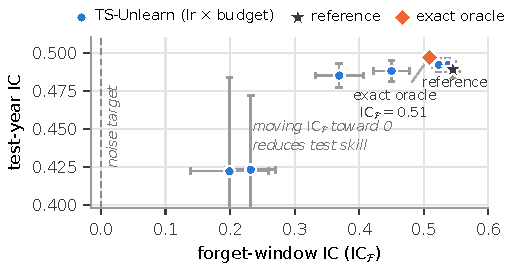
\includegraphics[width=0.92\columnwidth]{figs/fig_two_definitions}
\caption{The oracle and noise targets, compared on the Transformer
under the crisis-year deletion in the 2024 fold (\Lone). Each point
is one TS-Unlearn configuration (learning rate $\times$ budget),
averaged over ten seeds, with bars showing $\pm 1$ sd across seeds. The
dashed line marks the noise target, the diamond the exact
counterfactual, and the star the reference. The counterfactual has
higher test skill than the reference because deleting the crisis year
helps this model.}
\label{fig:twodefs}
\end{figure}

\begin{figure}[t]
\centering
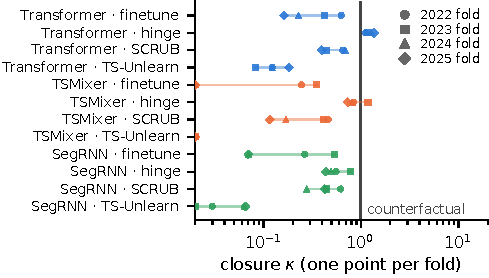
\includegraphics[width=0.92\columnwidth]{figs/fig_methods}
\caption{Closure $\gapclosed$ for each deployable
architecture-method pair on the crisis-year deletion (\Lone, 10
seeds, every method at its fixed a-priori hyperparameters), one
marker per fold, with a thin line connecting a pair's four folds. A
pair substitutes for the oracle only where its markers sit at the
counterfactual line. Values at or below zero are clipped to the
left edge of the log axis.}
\label{fig:methods}
\end{figure}

\subsection{Substitution for the oracle}

Figure~\ref{fig:methods} evaluates the four methods on the three
deployable architectures. The two non-deployable ones are omitted
from the figure. Each row is one architecture-method pair, with one
marker per fold. The test year plays no part in the closure. What
changes across folds is the training window and the position of
2020 inside it. Tightly clustered markers are a method that tracks
the oracle wherever the window sits. Scattered markers are a method
whose forgetting depends on the window it is applied to. The
vertical line at $\gapclosed = 1$ marks the counterfactual. In any
single fold, several pairs look adequate. Across all four, only
one pair stays close to the counterfactual line. The hinge on
TSMixer reaches closures of $0.74$ to $1.18$, crossing the line
from both sides and never straying from it by more than a quarter
of the gap, at no measurable cost in test skill. The hinge on the Transformer is second best; it
always overshoots, but never by more than half the gap. No other
pair stays within half the gap in every fold. For finetune, the
hinge, and SCRUB, the common failure is under-forgetting rather
than damage to the model.

TS-Unlearn fails at both of its budgets. Figure~\ref{fig:methods}
runs every method at the fixed protocol budget, and at that budget
TS-Unlearn forgets almost nothing, with
closures of $0.2$ or less on every architecture. The fixed budget
is not even harmless. In the bear-market fold, TS-Unlearn's test
skill falls $0.07$--$0.13$ IC short of the oracle and below the
reference itself, so it damages the model while forgetting almost
nothing. The sweep of
Figure~\ref{fig:twodefs} raised that budget deliberately, and there
it overshoots the counterfactual and destroys the model. A method
aimed at the noise target has no useful stopping point between the
two.

The rankings do not transfer across architectures. The same hinge
under-forgets on SegRNN, brackets the counterfactual on TSMixer,
and overshoots on the Transformer. On the non-deployable pair,
summarized in Table~\ref{tab:method_choice} and reported in full in
the released artifacts, the failures grow. The hinge
overshoots about fivefold on iTransformer, and SCRUB spans two
orders of magnitude across seeds on PatchTST, where the best-method
criterion itself degenerates: the method nearest the counterfactual
is the one that barely forgets. Nothing we measured
predicts which architecture a method will serve, and in particular
it is not the architecture with the largest memorization gap.

The fold scatter follows no rule either. Which fold lands high and
which lands low changes from pair to pair, so no fold-dependent
rule of thumb corrects a method's bias. The oracle's own gap for
the 2020 deletion varies by less than half across folds on the
deployable architectures, while the method scatter crosses from one
side of the counterfactual to the other, so the scatter comes from
the methods themselves, not from the yardstick.
Table~\ref{tab:method_choice} lists, for each architecture, the
best method under its worst fold.

The practical conclusion is that the oracle cannot be bypassed. A
closure of $1$ is defined by the oracle's fit to the removed year,
so without retraining a model owner cannot locate the target a
method is supposed to hit. The one combination that reaches the
target, the hinge on TSMixer, stops at a margin that must be set
from exactly that quantity. The figure shows that no substitute
locates the target either. Another architecture's result does not
transfer, another window position's result does not transfer, and
the memorization gap does not predict it. Validation against one's
own oracle is the only trustworthy acceptance test. It must be
repeated as the window slides, and at this scale each run costs
minutes.

\begin{table}[t]
\caption{The best method per deployable architecture, selected to
minimize the maximum $|\gapclosed-1|$ across folds. The closure range
spans the four folds. Skill cost is the worst-fold decrease in test IC
relative to the paired oracle, and the last column is wall-clock
cost relative to retraining.}
\label{tab:method_choice}
\centering
\footnotesize
\begin{tabular}{llccc}
\toprule
Architecture & Best method & Closure $\gapclosed$ & Skill cost & Cost \\
\midrule
TSMixer & hinge & $0.74$--$1.18$ & $0.004$ & $0.4\times$ \\
Transformer & hinge & $1.12$--$1.36$ & $0.011$ & $0.4\times$ \\
SegRNN & hinge & $0.44$--$0.79$ & $0.004$ & $0.2\times$ \\
\bottomrule
\end{tabular}
% Verified 2026-08-08 from the grid (worst-fold |kappa-1| criterion):
% hinge is the best on all three deployable archs; SCRUB on
% iTransformer confirmed. PatchTST's mechanical winner is TS-Unlearn
% at kappa 0.07-0.17, i.e. closest to 1 only because it barely
% forgets; 'none reliable' is the honest entry. Costs are mean method
% seconds over the era-2020 cells divided by the median oracle
% seconds of the same architecture and fold.
\end{table}

\section{RQ3: Can Deletion Be Audited?}\label{sec:rq3}

An auditor receives a model and must decide whether it behaves as
if it had trained on the deleted era. The audit of
Section~\ref{sec:method} compares two populations of ten seeds
each, references trained with the era and oracles retrained without
it, on their fit to the deleted windows. The separation $d'$ is the
standardized distance between the two populations. Near zero, the
populations overlap, and deletion cannot be certified from
behaviour. We ask whether the audit succeeds at the level of an
era, whether it succeeds at the level of a single training window,
and what treating overlapping windows as independent does to its
confidence.

\begin{figure}[t]
\centering
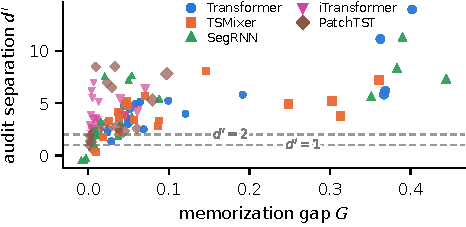
\includegraphics[width=0.92\columnwidth]{figs/fig_audit}
\caption{Audit separation $d'$ against the memorization gap $G$
for all 100 cells of architecture, deleted year, and fold (\Lone).
Crisis-year points are drawn larger, and the dashed lines mark
$d' = 1$ and $d' = 2$. All five architectures appear: an auditor
cannot presume the audited model is deployable, and the unverifiable
cells concentrate among the weak absorbers.}
\label{fig:audit}
\end{figure}

\subsection{Era-level auditing}

Figure~\ref{fig:audit} reports the audit in all 100 cells of
architecture, deleted year, and fold, instantiating the population
auditor of membership inference~\cite{carlini2022lira}. Each point
places one cell by its memorization gap from Section~\ref{sec:rq1}
on the horizontal axis and its audit separation on the vertical
axis. The figure therefore asks whether what a model memorized
decides what an auditor can see.

Across the grid the separation spans $-0.4$ to $14.0$. Removing the
crisis year from a heavy memorizer separates the two populations
completely. Removing a low- to medium-volatility year from a weak
memorizer leaves them indistinguishable from chance. What decides
the outcome is memorization. Separation rises with the gap across
the grid, and every cell the auditor cannot resolve is one where
the model had memorized almost nothing. Seventeen per cent of the
cells fall below $d' = 2$.

A legitimate deletion can therefore be unverifiable. The model did
not keep the data. It never memorized enough of it for the absence
to leave a trace. Auditability is a property of what was learned,
not of what was deleted, and a null audit is not evidence of
compliance.

\subsection{Window-level auditing}

A record-level right to erasure would require the audit to work on
a single training window. We therefore score each window separately
and ask how often the reference fits a window better than its own
oracle. The chance level of this win rate is one half. The win rate
stays near chance everywhere. Its median is just above one half,
and the best cell in the grid reaches only $0.69$. The win rate
rises with memorization, as the era-level separation does, but
never far enough to certify anything about a single window.
Whatever granularity a data contract names, it cannot be the
GDPR-style single record~\cite{gdpr2016}.

\subsection{Overlapping windows and audit power}

The window counts overstate the audit's evidence unless their
dependence is respected. Each forget day contributes about 480
windows, one per stock, and within a day those windows share one
market cross-section. The day mean therefore carries almost all of
the information, and the effective sample is the days, not the
windows. Treating windows as independent records inflates the audit
statistic by a median factor of $1.9$ across the grid, before any
window-level multiplicity is counted. HAC standard errors on panel
audit statistics are mandatory, not cosmetic.

Two further facts bound what an audit can promise. Extra forget
data does not buy power past the dispersion of the gap across
retraining seeds, which no amount of data lowers. And the minimum
detectable gap of the daily audit statistic, derived in the
released protocol, should accompany any audit verdict.

\section{Conclusion}\label{sec:conclusion}

Deleting a clean, legitimate year of market data is a gain, not a
cost, for every deployable architecture, in all four folds. Seeing
this took the unlearning literature's missing ground truth, which
this task makes affordable. The findings form one picture. What
``delete year $E$'' means must be fixed on a membership lattice,
and strictness has a measurable price. Exact deletion moves little
in calm markets, is two-sided under stress, and splits on a
standard volatility benchmark. One of the twelve deployable
architecture-method pairs brackets the oracle, and on the rest
nothing short of retraining does. The right target is the
counterfactual, which still predicts the deleted year. Deletion is
auditable only when the model memorized the era, so a null audit is
not evidence of compliance.

\textbf{Practice.} ``Licensee shall cease use of the Data''
under-specifies model obligations. A contract should name three
things. The first is the membership level, because strictness
changes both the surrendered data and the measured memory
(Table~\ref{tab:levels}). The second is the comparison standard,
which is equivalence to the retrained counterfactual
(Eq.~\ref{eq:compliance}) and not inability to predict. The third
is the audit granularity, which the era level can support and the
single record cannot. Three cautions complete the picture. Do not
quantize after approximate unlearning. At LLM scale, quantization
restores up to $83\%$ of what was unlearned, while exact retraining
is immune~\cite{zhang2025quantfail}. Read over-forgetting as
evidence of post-hoc treatment rather than thoroughness, because
the retrained counterfactual never over-forgets. And a model with
no alpha can still fail an audit, because memorization is a
property of fitting, not of skill.

\textbf{Limitations.} All claims are regime-contrast claims on one
liquid US equity panel and one task, and architecture-level
statements rest on five models in which test skill and memorization
are collinear. We can order how much of each era a model memorized,
but we cannot predict a deletion's sign from that ordering, because
the correlation between memorization and effect is carried by the
crisis year alone. Why 2020 in particular inverts the sign is not
something one crisis can answer. Every window is a fixed five years
and every architecture carries one configuration, selected before
any deletable era. Expanding windows and other selection rules are
left to future work. Protocol, configurations, per-cell artifacts,
and verification scripts are released, and any cell reproduces from
the frozen environment in one command.


\bibliographystyle{ACM-Reference-Format}
\bibliography{refs}

\end{document}
